\label{sec:CNN}
Convolutional Neural Networks (CNNs) are neural networks that use assumptions about the local relationships between neigboring pixels in order to predict the content of an input image. For this analysis, content prediction is simplified to a general classification of whether the image comes from a dihiggs or QCD event. The fundamental elements of any convolutional network are convolutional layers and pooling layers. Convolutional layers use filters that perform non-linear combinations of neighboring pixels within the filter size, and pooling layers aggregate information by grouping neighboring pixels by either their maximum or average values. After some number of these layers, the output is flattened into a one-dimensional vector, and this flattened vector is pushed through a set of feed-forward layers in order to make a final output prediction. 

Many previous papers have explored the training convolutional networks using low-level measured quantities (e.g. tracks and calorimeter deposits) in high energy physics in the context of object identification [CITATION NEEDED]. This paper extends the application to event-level identification. Using low-level quantities removes the need to reconstruct objects like jets since no higher-level quantites (e.g. dijet masses) are needed; only the detector-level measurements are required for classification. The performance of four convolutional networks are studied in the context of dihiggs identification. The first network uses a 3-layer image composed of energy/momentum weighted tracks, electromagnetic calorimeter deposits, and hadronic calorimeter deposits. The second network uses the same three layers but appends additional global information to the flattened vector after image processing and before the fully connected layers. Figures~\ref{fig:cnn_nominal} and \ref{fig:cnn_hybrid} depict both network strucutres. The third and fourth networks follow the same pattern as the previous two but with the addition of two image layers corresponding to impact parameter-weighted track information (both longitudinal and transverse).

\begin{figure}[!h] 
\begin{center}
\includegraphics*[width=0.75\textwidth] {CNN/figures/nominalCNN.png}
\caption{Structure of the nominal convolutional neural network. The input images are fed through two convolutional layers and a single max-pooling layer before being flattened into a one-dimensional vector. The flattened vector is then fed through one fully connected layer, a batch normalization layer, and a final fully connected layer before a final prediction is made.}
  \label{fig:cnn_nominal}
\end{center}
\end{figure}

\begin{figure}[!h] 
\begin{center}
\includegraphics*[width=0.75\textwidth] {CNN/figures/hybridCNN.png}
\caption{Structure of the hybrid convolutional neural network. The input images are fed through two convolutional layers and a single max-pooling layer before being flattened into a one-dimensional vector. Scaled user-specified variables (e.g. $H_{T}$) are then concatenated with the flattened image vector. The concatenated vector is then fed through one fully connected layer, a batch normalization layer, and a final fully connected layer before a final prediction is made.}
  \label{fig:cnn_hybrid}
\end{center}
\end{figure}

In order to produce coherent images, the center of mass and the center of momentum for each event are calculated. All consituents are then boosted longitudinally into the center of mass of the event and rotated in phi to the center of momentum. At the end, each image layer corresponds to a 31x31 pixel grid centered on the total activity in the event. Figure~\ref{fig:cnn_avgQCD} shows an average QCD image and Figure~\ref{fig:cnn_avgDihiggs} shows an average signal image. While the layers in each figure closely resemble one another, they do contain different information, and variations are visible. More importantly, the average QCD image differs significantly from the average dihiggs image. 

\begin{figure}[!h] 
\begin{center}
  \subfloat[]{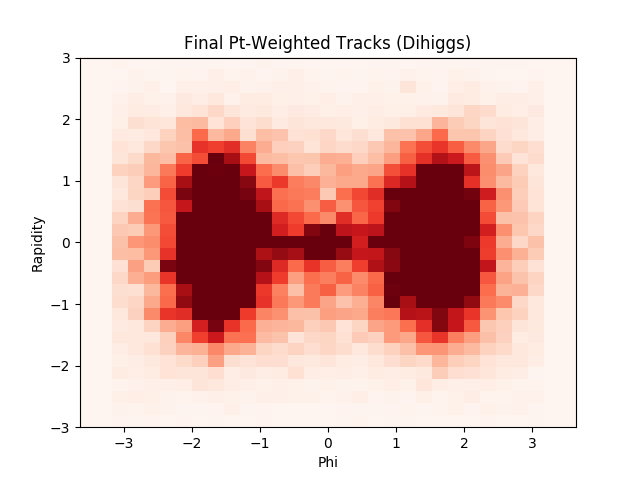
\includegraphics[width = 2in]{CNN/figures/images/qcd/Tracks_Dihiggs_Final_Pt-Weighted}} 
  \subfloat[]{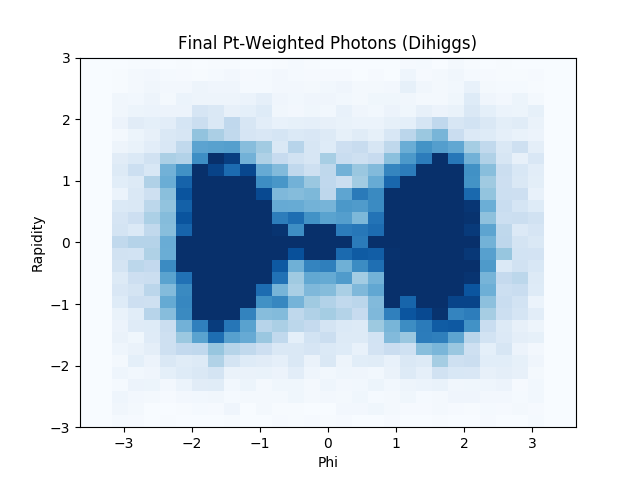
\includegraphics[width = 2in]{CNN/figures/images/qcd/Photons_Dihiggs_Final_Pt-Weighted}}
  \subfloat[]{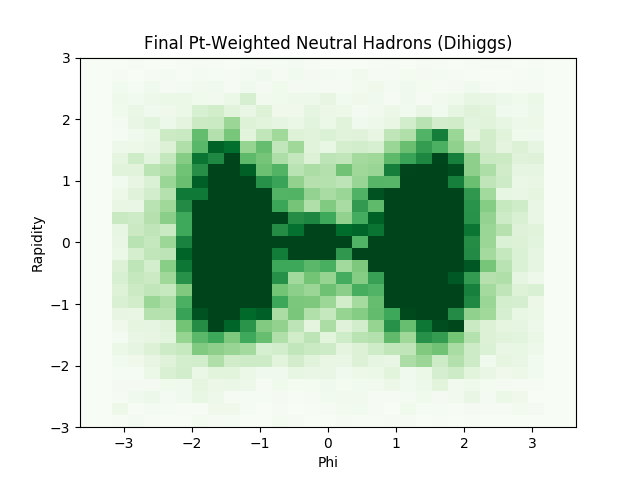
\includegraphics[width = 2in]{CNN/figures/images/qcd/NeutralHadrons_Dihiggs_Final_Pt-Weighted}} \\
  \subfloat[]{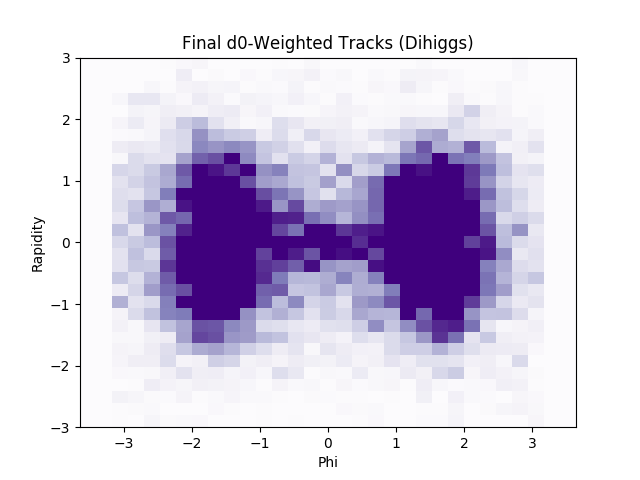
\includegraphics[width = 2in]{CNN/figures/images/qcd/Tracks_Dihiggs_Final_d0-Weighted}} 
  \subfloat[]{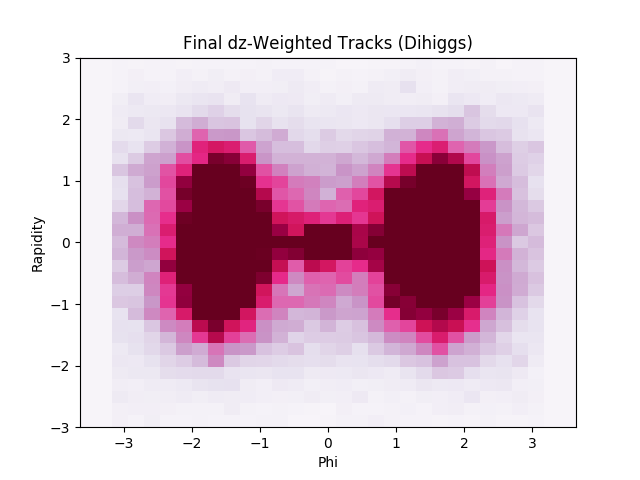
\includegraphics[width = 2in]{CNN/figures/images/qcd/Tracks_Dihiggs_Final_dz-Weighted}} 
\caption{Average QCD image showing (a) $p_{\textrm{T}}$-weighted tracks, (b) $E_{\textrm{T}}$-weighted ECAL deposits, (c) Et-weighted HCAL deposits, (d) transverse impact parameter-weighted tracks, (e) longitudinal impact parameter-weighted tracks.}
\end{center}
\label{fig:cnn_avgQCD}
\end{figure}

\begin{figure}[!h] 
\begin{center}
  \subfloat[]{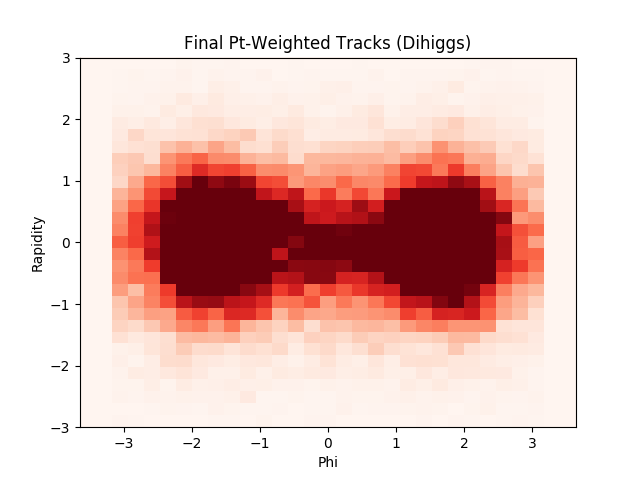
\includegraphics[width = 2in]{CNN/figures/images/hh/Tracks_Dihiggs_Final_Pt-Weighted}} 
  \subfloat[]{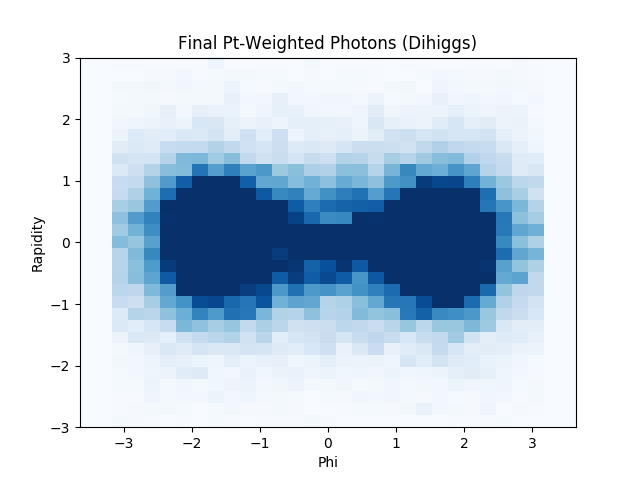
\includegraphics[width = 2in]{CNN/figures/images/hh/Photons_Dihiggs_Final_Pt-Weighted}}
  \subfloat[]{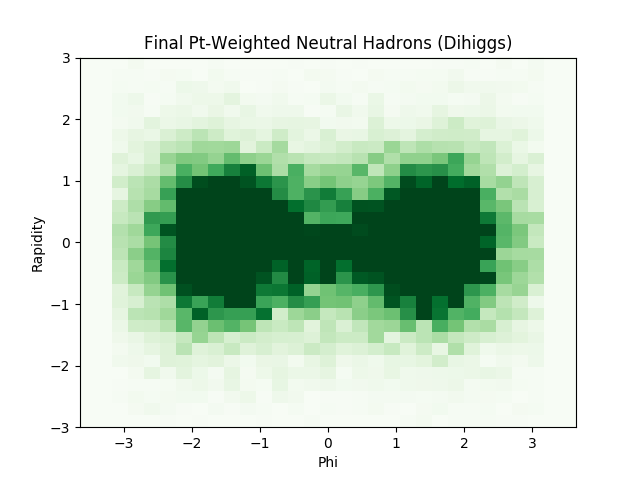
\includegraphics[width = 2in]{CNN/figures/images/hh/NeutralHadrons_Dihiggs_Final_Pt-Weighted}} \\
  \subfloat[]{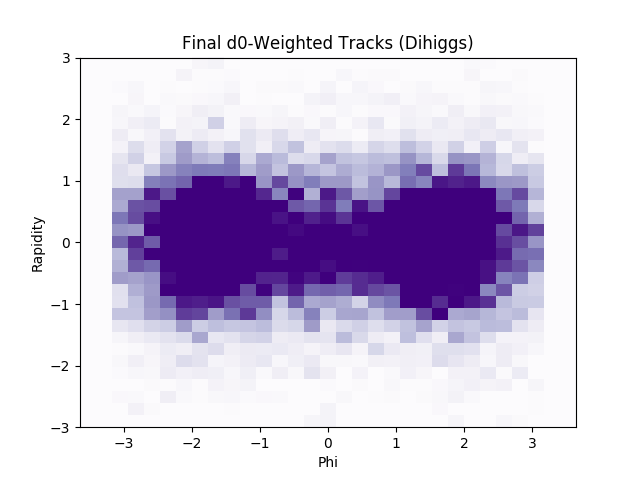
\includegraphics[width = 2in]{CNN/figures/images/hh/Tracks_Dihiggs_Final_d0-Weighted}} 
  \subfloat[]{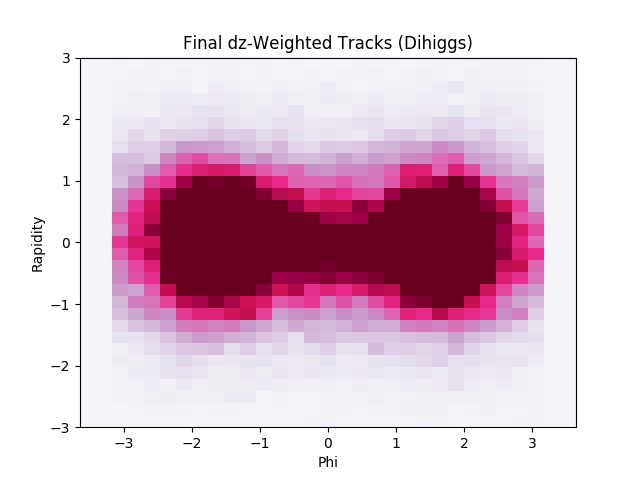
\includegraphics[width = 2in]{CNN/figures/images/hh/Tracks_Dihiggs_Final_dz-Weighted}} 
\caption{Average dihiggs image showing (a) pt-weighted tracks, (b) Et-weighted ECAL deposits, (c) Et-weighted HCAL deposits, (d) transverse impact parameter-weighted tracks, (e) longitudinal impact parameter-weighted tracks.}
\end{center}
\label{fig:cnn_avgDihiggs}
\end{figure}

As shown in Figures~\ref{fig:cnn_nominal} and \ref{fig:cnn_hybrid}, the CNN network structure uses two sequential 2D convolutional layers each with 16 3x3 filters, one max-pooling layer with a 2x2 window, a flattening of the outputs, two 64-node fully connected hidden layers, and one output layer for making the final prediction. As previously described, two of the networks append additional high level variables (scalar sum of transverse hadronic energy, number of jets, and number of $b$-tags) after the flattening and before the image information is fed through the fully connected layers. Optimal significances for each network are shown in Table~\ref{tab:cnnResults} and the output signal predictions and ROC for the 5-color network with high-level inputs are shown in Figure~\ref{fig:cnn_preds}.

\begin{table}[h!]
\label{tab:cnnResults}
  \begin{center}
    \begin{tabular}{|l|c|c|} % <-- Alignments: 1st column left, 2nd middle and 3rd right, with vertical lines in between
      \hline\hline
      \textbf{Method} & Best $S/\sqrt{B}$ & AUC \\
      \hline
      Tracks+HCAL+ECAL & 1.77 $\pm$ 0.01 & 0.818 \\
      Tracks+HCAL+ECAL + high-level & 2.12 $\pm$ 0.01 & 0.846 \\
      Tracks+HCAL+ECAL+D0+DZ & 2.45 $\pm$ 0.02 & 0.863 \\
      Tracks+HCAL+ECAL+D0+DZ + high-level & 2.86 $\pm$ 0.03 & 0.882 \\

      \hline\hline
    \end{tabular}
    \caption{Normalized to full HL-LHC dataset of 3000 fb$^{-1}$}
  \end{center}
\end{table}


\begin{figure}[!h] 
\begin{center}
  \subfloat[]{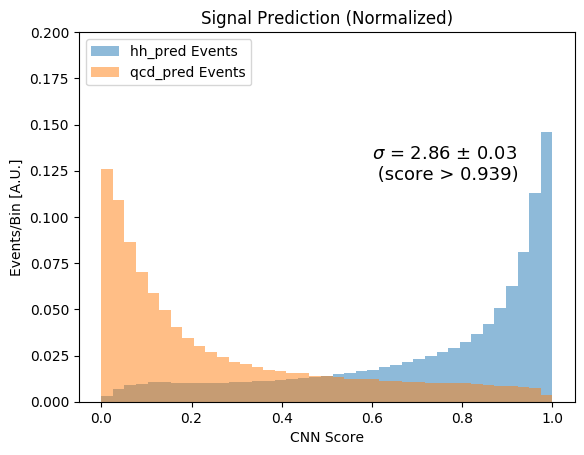
\includegraphics[width = 3in]{CNN/figures/5color_0PU_pix31_addHT-nJets-nBTags_2Conv16-16_one2DPool_EqualSamples/signal_CNNScore_norm}} 
  \subfloat[]{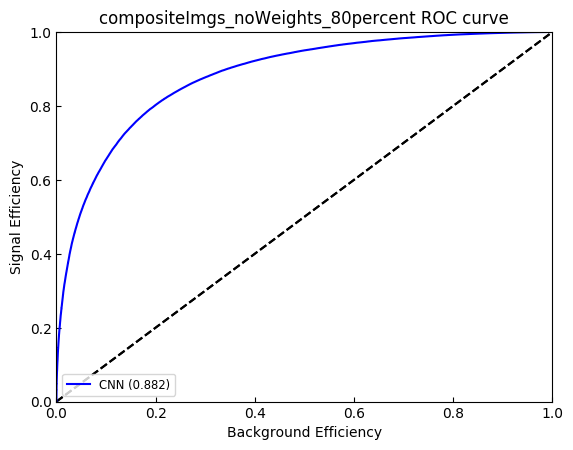
\includegraphics[width = 3in]{CNN/figures/5color_0PU_pix31_addHT-nJets-nBTags_2Conv16-16_one2DPool_EqualSamples/compositeImgs_noWeights_80percent_ROC}}\\
\caption{(Right) signal prediction for the 5-color convolutional network with additional high-level inputs, (Left) ROC for the 5-color convolutional network with additional high-level inputs.}
\end{center}
\label{fig:cnn_preds}
\end{figure}

